\chapter{光的标量模型}\label{ch:b2:scalar-light-model}

让两只手电照在同一面墙上，光斑的亮度只是加倍；
让同一台激光器发出的两束光照在墙上，光斑则分裂成
明暗相间的条纹。手电的光强相加，激光束的振幅相加——
而接下来各章中的每一台干涉仪、全息图和衍射光栅，都依赖于
判断光在何时表现出哪一种行为。本章建立相应的工具：
把光视为带有相位的\emph{标量}波，
用\emph{\omterm{def:b2:scalar-light-model:path}{光程}}沿光线度量该相位，
光源发光的方式——以短\omterm{prop:b2:scalar-light-model:coherence}{波列}的形式发出，其
\emph{\omterm{prop:b2:scalar-light-model:coherence}{相干长度}}决定两列波能否干涉——
和探测器记录光的方式：对数十亿个周期取平均，
只保留强度。

\section{作为标量波的光}

\begin{definition}[光的标量模型；单色波]\label{def:b2:scalar-light-model:scalar}
\index{光的标量模型}\index{振动（光学）}\index{单色波}
在大多数波动光学问题中，光的矢量性质不起作用（
叠加的波具有同一偏振方向，或光是非偏振的，
其偏振平均抵消）：场被一个实的
\emph{标量振动}
\[
s(M, t) = a(M)\cos\bigl(\omega t - \varphi(M)\bigr) ,
\]
在每一点处具有振幅 $a(M)$ 与相位 $\varphi(M)$，二者
都在波长尺度上缓慢变化。\emph{单色}波
只有一个 $\omega$：这是一种理想化，因为实际光源
发出的光占据一段频率范围。可见光：波长 $\lambda_0$ 从 $400$ 到
\qty{750}{nm}（真空中），频率 $\nu = c/\lambda_0$ 从 $7.5 \times 10^{14}$ 到 $4 \times 10^{14}$ Hz，
周期约为 \qty{2}{fs}。
\end{definition}

\begin{definition}[光程与相位]\label{def:b2:scalar-light-model:path}
\index{光程}\index{相位（光学）}\index{波前}\index{马吕斯–杜平定理}
在折射率为 $n$ 的介质中，波速为 $c/n$，波长为
$\lambda_0/n$。沿从 $A$ 到 $B$ 的曲线，\emph{光程}为
\[
(AB) = \int_A^Bn\,\dd s ,
\]
则\omterm{def:b2:scalar-light-model:scalar}{单色波}沿一条光线
从 $A$ 到 $B$ 传播时积累的相位为
\[
\varphi(B) - \varphi(A) = \frac{2\pi}{\lambda_0}\,(AB) = \omega\,\tau_{AB} ,
\]
其中 $\tau_{AB}$ 为传播时间。\emph{波前}是
等相位的曲面；在各向同性介质中，几何光学的光线
与波前垂直（马吕斯–杜平定理），且两波前之间的
光程沿每一条光线都相同。
\end{definition}

\begin{proof}[论证]
相位每前进 $2\pi$，对应一个局部波长 $\lambda_0/n$，
故每个线元的相位增量为 $2\pi n\,\dd s/\lambda_0$（线元为 $\dd s$），沿光线求和。波
$a\cos(\omega t - \varphi)$ 是\omterm{thm:b2:waves-on-strings:equation}{波动方程}的解，其中能量
沿 $\operatorname{\vect{grad}}\varphi$ 方向传播，且与
$\varphi = $ 常量的面垂直：这正是光线，而“\omterm{def:b2:scalar-light-model:path}{光程}
在两\omterm{def:b2:scalar-light-model:path}{波前}之间相同”的陈述，
倒过来读，就是\omterm{def:b2:scalar-light-model:path}{波前}的定义。完整定理（它在反射与
折射下仍成立）在本阶段不加证明地承认。
\end{proof}

\begin{example}[严格成像；作为相位板的透镜]\label{ex:b2:scalar-light-model:lens}
\index{严格成像}\index{薄透镜（相位）}
一个点光源 $A$ 经理想的（\omterm{ex:b2:scalar-light-model:lens}{严格成像}的）仪器成像于 $A'$：
从 $A$ 到 $A'$ 的所有光线具有\emph{相同的\omterm{def:b2:scalar-light-model:path}{光程}}——
沿各条光线到达的波在 $A'$ 处同相，这正是它们
在该处叠加成一个亮点。对焦距为 $f$ 的薄透镜，
这是关于相位的一个论断：沿光轴入射的平面波
必须以汇聚于焦点 $F'$ 的\omterm{prop:b2:sound-waves:spherical}{球面波}射出；由于
中心位于距离 $f$ 处的\omterm{prop:b2:sound-waves:spherical}{球面波}，在距光轴 $r$ 处，
其相位比轴上的值超前 $2\pi r^2/2\lambda f$（近轴
近似，$\sqrt{f^2 + r^2} \approx f + r^2/2f$），透镜必须
使波\emph{延迟} $\varphi_L(r) = -\pi r^2/\lambda f$：透镜在
中心处更厚，厚出的量恰好使所有到 $F'$ 的\omterm{def:b2:scalar-light-model:path}{光程}
相等。透镜是一块相位板；全息图或液晶显示器
若施加相同的相位分布，即为一个透镜。
\end{example}

\begin{omfigure}
\begin{tikzpicture}[font=\small, x=1cm, y=1cm, >=Stealth]
  \begin{scope}
    \foreach \x in {-3.0,-2.4,-1.8} \draw[omDef, thick] (\x,-1.5) -- (\x,1.5);
    \draw[thick, fill=omExo!20] (0,0) ellipse (0.25 and 1.6);
    \draw[omDef, thick] (1.0,1.25) arc[start angle=125, end angle=235, x radius=1.9, y radius=1.5];
    \draw[omDef, thick] (1.7,1.0) arc[start angle=130, end angle=230, x radius=1.4, y radius=1.3];
    \draw[omDef, thick] (2.35,0.7) arc[start angle=135, end angle=225, x radius=1.0, y radius=1.0];
    \fill (3.2,0) circle (1.6pt); \node[font=\footnotesize] at (3.4,-0.3) {$F'$};
    \draw[omThm, ->] (-3.2,0.9) -- (-0.4,0.9); \draw[omThm, ->] (0.3,0.9) -- (3.1,0.05);
    \draw[omThm, ->] (-3.2,-0.9) -- (-0.4,-0.9); \draw[omThm, ->] (0.3,-0.9) -- (3.1,-0.05);
    \draw[omThm, ->] (-3.2,0) -- (3.1,0);
    \node[font=\footnotesize] at (0,-2.1) {平面波前 $\to$ 球面波：透镜延迟中心};
  \end{scope}
  \begin{scope}[xshift=9.0cm]
    \fill[omExo!20] (-1.0,-1.4) rectangle (1.0,1.4); \draw[thick] (-1.0,-1.4) -- (-1.0,1.4) (1.0,-1.4) -- (1.0,1.4);
    \foreach \x in {-2.8,-2.2,-1.6} \draw[omDef, thick] (\x,-1.2) -- (\x,1.2);
    \foreach \x in {-0.7,-0.3,0.1,0.5,0.9} \draw[omDef, thick] (\x,-1.2) -- (\x,1.2);
    \foreach \x in {1.6,2.2,2.8} \draw[omDef, thick] (\x,-1.2) -- (\x,1.2);
    \node[font=\footnotesize] at (0,1.7) {$n$: $\lambda_0/n$}; \node[font=\footnotesize] at (-2.2,1.7) {$\lambda_0$};
    \node[font=\footnotesize] at (0,-2.1) {光程 $(AB) = \int n\,\dd s$};
  \end{scope}
\end{tikzpicture}

{\small 左：薄透镜将平面\omterm{def:b2:scalar-light-model:path}{波前}变为\omterm{prop:b2:sound-waves:spherical}{球面波}前，
会聚于焦点——到 $F'$ 的所有\omterm{def:b2:scalar-light-model:path}{光程}均相等。右：
玻璃内波长缩短为 $\lambda_0/n$，相位
前进得更快：\omterm{def:b2:scalar-light-model:path}{光程}相当于几何长度的 $n$ 倍。}
\end{omfigure}

\section{光的发射：相干性}

\begin{proposition}[波列；相干时间与相干长度]\label{prop:b2:scalar-light-model:coherence}
\index{波列}\index{相干时间}\index{相干长度}\index{谱宽}
经典光源（火焰、灯、恒星）是大量原子的集合，
每个原子在随机时刻、以随机相位发出一段短促的
\emph{\omterm{prop:b2:scalar-light-model:coherence}{波列}}（持续时间 $\tau_c$）：光源在一点产生的振动
在 $\tau_c$ 内保持相位稳定，随后跳变。一段
持续时间为 $\tau_c$ 的\omterm{prop:b2:scalar-light-model:coherence}{波列}并非单色：其谱覆盖一段频率
范围 $\Delta\nu \approx 1/\tau_c$（傅里叶互易关系，在本阶段不加证明地承认：有限长的
正弦波不可能只有单一频率）。\emph{\omterm{prop:b2:scalar-light-model:coherence}{相干时间}}
$\tau_c$ 与\emph{\omterm{prop:b2:scalar-light-model:coherence}{相干长度}}
\[
\ell_c = c\,\tau_c \approx \frac c{\Delta\nu} = \frac{\lambda^2}{\Delta\lambda}
\]
表征光源：白光 $\Delta\lambda \approx \qty{300}{nm}$，$\ell_c
\approx \qty{1}{\micro m}$；光谱灯（$\Delta\lambda \sim \qty{0.01}{nm}$），$\ell_c \sim
\qty{3}{cm}$；激光器则为米至千米量级。两列由同一光源导出的波
只有当\omterm{def:b2:scalar-light-model:path}{光程}差小于
$\ell_c$ 时才能干涉——超出此范围，它们分属不同的\omterm{prop:b2:scalar-light-model:coherence}{波列}，
相位彼此无关。
\end{proposition}

\begin{proof}
由 $\ell_c = c/\Delta\nu$、$|\Delta\nu/\nu| = |\Delta\lambda/\lambda|$ 及 $\nu = c/\lambda$ 可得 $\ell_c =
\lambda^2/\Delta\lambda$。\omterm{prop:b2:scalar-light-model:coherence}{谱宽}本身有以下物理成因：
自然展宽（辐射阻尼，见\cref{ch:b2:dipole-radiation}）、
原子热运动造成的多普勒展宽、碰撞——这些因素均
会缩短\omterm{prop:b2:scalar-light-model:coherence}{波列}。
\end{proof}

\begin{omfigure}
\begin{tikzpicture}
\begin{axis}[omaxis, axis x line=middle, axis y line=none, width=13.6cm, height=3.6cm,
    xmin=0, xmax=60, ymin=-1.4, ymax=1.6, xtick=\empty, samples=800, xlabel={$t$},
    xlabel style={at={(axis description cs:1.0,0.5)}, anchor=west}]
  \addplot[omDef, thick, domain=0:14] {cos(deg(2.2*x))};
  \addplot[omDef, thick, domain=14:31] {cos(deg(2.2*x)+110)};
  \addplot[omDef, thick, domain=31:42] {cos(deg(2.2*x)+240)};
  \addplot[omDef, thick, domain=42:60] {cos(deg(2.2*x)+40)};
  \draw[omThm, <->] (axis cs:14,1.35) -- (axis cs:31,1.35) node[midway, above, font=\scriptsize] {$\tau_c$};
  \draw[omThm, dashed] (axis cs:14,-1.2) -- (axis cs:14,1.2);
  \draw[omThm, dashed] (axis cs:31,-1.2) -- (axis cs:31,1.2);
  \draw[omThm, dashed] (axis cs:42,-1.2) -- (axis cs:42,1.2);
\end{axis}
\end{tikzpicture}

{\small 经典光源产生的振动：一系列
持续时间为 $\tau_c$ 的\omterm{prop:b2:scalar-light-model:coherence}{波列}，相邻\omterm{prop:b2:scalar-light-model:coherence}{波列}之间有随机的相位跳变；两
份副本只有在延迟小于 $\tau_c$ 时才能发生干涉。}
\end{omfigure}

\begin{remark}[两个光源与同一光源]\label{rem:b2:scalar-light-model:twosources}
\index{非相干光源}
两盏不同的灯（或两个不同的原子）发出的\omterm{prop:b2:scalar-light-model:coherence}{波列}具有
彼此独立的随机相位：它们的相对相位每隔 $\tau_c
\sim \qty{1e-9}{s}$ 变化一次，比任何眼睛或照相机的响应快百万倍——
干涉项的平均值为零，强度
直接相加。干涉要求两列波\emph{记住相同的
相位跳变}：即由同一列波分出的两份副本，
（双缝、两面镜子、薄膜的两个表面）分开后重新叠加，且
延迟小于 $\tau_c$。激光器的\omterm{prop:b2:scalar-light-model:coherence}{波列}可持续微秒量级甚至更久，
这一要求被大大放宽，却从未被取消。
\end{remark}

\section{探测器与强度}

\begin{proposition}[探测器测量什么]\label{prop:b2:scalar-light-model:intensity}
\index{强度（光学）}\index{探测器（光学）}\index{光子通量}
各类光探测器——眼睛（响应时间 $\sim\qty{0.1}{s}$）、
照相胶片、CCD 像素（\qty{1}{ms}）、光电二极管（\qty{1}{ns}）——
其响应时间远长于周期（$10^{-15}$ s），并
给出\emph{强度}，即振动平方的
时间平均：
\[
I = K\,\langle s^2\rangle = \tfrac12K\,a^2 ,
\]
（$K$ 为常数，常略去；$I$ 正比于辐照度，
以 \unit{W/m^2} 计）。绝对水平仅在一点上起作用：光
以能量为 $h\nu$ 的光子形式到达，探测器平均每
单位面积、单位时间计数 $I/h\nu$ 个光子。
\end{proposition}

\begin{proof}
$\langle\cos^2(\omega t - \varphi)\rangle = \tfrac12$，只要时间间隔远大于
$2\pi/\omega$ 即成立。光子的内容见本科一年级分册的最后一章；此处
正是标量波与量子理论的交汇点。
\end{proof}

\begin{example}[数量级]\label{ex:b2:scalar-light-model:orders}
一只 \qty{60}{W} 的灯泡辐射出 \qty{3}{W} 的可见光，在 \qty{2}{m} 处：
$I = 3/4\pi\cdot4 = \qty{60}{mW/m^2}$，$I/h\nu = 1.6 \times 10^{17}$ 个光子
每平方米每秒；每秒经 \qty{5}{mm} 瞳孔进入的光子为 $3 \times 10^{12}$ 个——
在眼睛的 \qty{0.1}{s} 内，毫无颗粒感的痕迹。
肉眼所能看到的最暗恒星每秒射入
瞳孔的光子约 $\sim 10^3$ 个；视杆细胞只需寥寥数个光子即可响应。日光：\qty{1}{kW/m^2}，$3 \times 10^{21}$
个光子，每平方米每秒。
\end{example}

\begin{omfigure}
\begin{tikzpicture}[font=\small, x=1cm, y=1cm, >=Stealth]
  \draw[->, thick] (0,0) -- (12.6,0) node[right, font=\footnotesize] {时间 (s)};
  \foreach \x/\l in {0/$10^{-15}$, 2/$10^{-13}$, 4/$10^{-11}$, 6/$10^{-9}$, 8/$10^{-7}$, 10/$10^{-5}$, 12/$10^{-3}$} {
    \draw (\x,-0.1) -- (\x,0.1); \node[font=\scriptsize, below] at (\x,-0.12) {\l};
  }
  \draw[omDef, very thick] (0,0.45) -- (0.4,0.45); \node[omDef, font=\footnotesize, anchor=west] at (0.5,0.45) {光学周期};
  \draw[omThm, very thick] (2.0,0.95) -- (6.0,0.95); \node[omThm, font=\footnotesize, anchor=west] at (6.1,0.95) {波列（灯）};
  \draw[omThm, very thick] (6.0,1.45) -- (10.0,1.45); \node[omThm, font=\footnotesize, anchor=west] at (10.1,1.45) {激光器};
  \draw[omProp, very thick] (6.0,1.95) -- (12.4,1.95); \node[omProp, font=\footnotesize, anchor=west] at (6.1,2.2) {探测器：光电二极管 $\to$ CCD $\to$ 眼睛（$10^{-1}$）};
\end{tikzpicture}

{\small 光学中的时间尺度：振动的周期、
经典光源与激光器\omterm{prop:b2:scalar-light-model:coherence}{波列}的持续时间，以及
探测器的响应时间——所有探测器都在许多
个周期内取平均，对灯光而言还需跨越许多个\omterm{prop:b2:scalar-light-model:coherence}{波列}。}
\end{omfigure}

\begin{remark}[相干叠加与非相干叠加]\label{rem:b2:scalar-light-model:superposition}
\index{相干叠加}\index{非相干叠加}
两个振动 $a_1\cos(\omega t - \varphi_1)$ 与 $a_2\cos(\omega t - \varphi_2)$ 在某一
点处叠加，给出 $s = s_1 + s_2$，并且
\[
I = \tfrac12K\bigl[a_1^2 + a_2^2 + 2a_1a_2\langle\cos(\varphi_1 - \varphi_2)\rangle\bigr] .
\]
若探测过程中相位差保持稳定
（\emph{相干}波）：$I = I_1 + I_2 + 2\sqrt{I_1I_2}\cos(\varphi_1 - \varphi_2)$，
其中的干涉项将在下一章研究。若相位差无规
漂移（\emph{非相干}波）：$\langle\cos\rangle = 0$，且 $I = I_1 +
I_2$ ——即普通火把。
\end{remark}

\begin{method}[光学问题的建立]\label{met:b2:scalar-light-model:method}
（1）将每列波写成 $a\cos(\omega t - \varphi)$，其中 $\varphi = 2\pi(\text{
光程})/\lambda_0$，自光源（或自共同\omterm{def:b2:scalar-light-model:path}{波前}）算起。（2）判断相干性：
是否来自同一光源，\omterm{def:b2:scalar-light-model:path}{光程}差 $< \ell_c$？若是，则将振幅相加
（用复数记法较为方便：$\underline s = a\eu^{\iu(\omega t - \varphi)}$，$I =
\tfrac12K|\underline s|^2$）；否则将强度相加。（3）对透镜和
反射镜，利用共轭点间的等\omterm{def:b2:scalar-light-model:path}{光程}，或采用
相位板图像。（4）换算为可测量的量：强度、
对比度、光子计数，并检查探测器在时间
与空间上的分辨率。
\end{method}

\section{练习}

\begin{exercise}[$\star$]\label{exo:b2:scalar-light-model:1}
一束波长为 \qty{600}{nm} 的光束穿过 \qty{1.0}{cm} 厚的玻璃（$n = 1.5$）。
求\omterm{def:b2:scalar-light-model:path}{光程}；玻璃内的波长数；与 \qty{1}{cm} 空气相比的附加相位和附加延迟；
使波相对于空气恰好延迟一个波长的
玻璃厚度。
\end{exercise}

\begin{exercise}[$\star$]\label{exo:b2:scalar-light-model:2}
求下列各光源的\omterm{prop:b2:scalar-light-model:coherence}{相干时间}和\omterm{prop:b2:scalar-light-model:coherence}{相干长度}：白光（$400$--\qty{750}{nm}）；钠灯
谱线，宽度 \qty{0.02}{nm}，中心波长 \qty{589}{nm}；红色发光二极管（\qty{630}{nm}，
$\Delta\lambda = \qty{25}{nm}$）；多模激光二极管（$\Delta\nu = \qty{100}{GHz}$）；
稳频激光器（$\Delta\nu = \qty{1}{kHz}$）。哪些光源能在\omterm{def:b2:scalar-light-model:path}{光程}差为
\qty{1}{mm} 时产生干涉条纹？\omterm{def:b2:scalar-light-model:path}{光程}差为 \qty{10}{m} 时呢？
\end{exercise}

\begin{exercise}[$\star$]\label{exo:b2:scalar-light-model:3}
求功率为 \qty{1}{mW}、波长为 \qty{650}{nm} 的激光笔每秒发出的光子数；
一只 \qty{100}{W} 灯泡（可见光部分 \qty{5}{W}，平均波长 \qty{550}{nm}）位于 \qty{3}{m} 处，每秒
穿过直径为 \qty{6}{mm} 的瞳孔的光子数；眼睛在 \qty{0.1}{s} 内接收的光子数；
该数的相对涨落 $1/\sqrt N$——光是否具有颗粒性？
\end{exercise}

\begin{exercise}[$\star$]\label{exo:b2:scalar-light-model:4}
一点光源距屏 \qty{1.0}{m}，$\lambda = \qty{500}{nm}$。求
屏中心与距轴 \qty{1}{cm} 处一点之间的\omterm{def:b2:scalar-light-model:path}{光程}差
（精确计算，再用近轴公式 $r^2/2d$）；所含
波长数；屏上\omterm{def:b2:scalar-light-model:path}{波前}的半径；离轴距离为多少时，
近轴公式的误差恰为一个波长？
\end{exercise}

\begin{exercise}[$\star\star$]\label{exo:b2:scalar-light-model:5}
\emph{透镜作为相位板。}（a）沿轴方向的平面波在薄透镜平面上具有
均匀的相位；经透镜后，相位为
$\varphi_L(r) = -\pi r^2/\lambda f$（相对于中心）。证明出射
\omterm{def:b2:scalar-light-model:path}{波前}在近轴近似下是半径为 $f$ 的球面，
球心位于 $F'$。（b）距透镜前 $d$ 处的点光源
发出的波在透镜平面上的相位为 $+\pi r^2/\lambda d$（相对于
中心）。证明经透镜后，波会聚于 $d'$，且
$1/d' = 1/f - 1/d$，即透镜公式。（c）平凸玻璃透镜的厚度分布
（$n = 1.5$，焦距 \qty{10}{cm}）为 $e(r) =
e_0 - r^2/2(n - 1)f$；求 $r = \qty{1}{cm}$ 处的垂度。（d）“菲涅耳透镜”将
轮廓每超过 $\lambda/(n - 1)$ 即折回：为何仍
能聚焦，以及为何只有一种颜色能被完美聚焦？
\end{exercise}

\begin{exercise}[$\star\star$]\label{exo:b2:scalar-light-model:6}
\emph{反射镜的\omterm{ex:b2:scalar-light-model:lens}{严格成像}。}反射镜须将沿其轴入射的
平面波会聚到点 $F$。（a）写出条件：
从平面\omterm{def:b2:scalar-light-model:path}{波前}经反射镜上每一点到 $F$ 的\omterm{def:b2:scalar-light-model:path}{光程}都相等，
并证明它确定抛物线 $y^2 = 4fx$，其焦点为 $F$。（b）为何球面镜只是
近似\omterm{ex:b2:scalar-light-model:lens}{严格成像}（将 $y^2 = 4fx$ 与
顶点附近半径为 $2f$ 的圆比较）？（c）对口径为 \qty{20}{cm} 的反射镜，
焦距 $f = \qty{1}{m}$，球面在边缘处的\omterm{def:b2:scalar-light-model:path}{光程}误差，以
\qty{500}{nm} 波长计。（d）为何射电望远镜能容忍
光学望远镜无法容忍的球面偏差？
\end{exercise}

\begin{exercise}[$\star\star$]\label{exo:b2:scalar-light-model:7}
\emph{费马原理。}从 $A$（在介质 $n_1$ 中）到 $B$（在
$n_2$ 中）经平面界面上一点 $P$ 的\omterm{def:b2:scalar-light-model:path}{光程}为 $n_1AP + n_2PB$。（a）
证明：当点 $P$ 满足
$n_1\sin\theta_1 = n_2\sin\theta_2$ 时，\omterm{def:b2:scalar-light-model:path}{光程}取驻值（极小）。（b）解释：相邻路径具有
相同的相位，沿这些路径的波因而相加，这正是光
“选择”笛卡儿射线的原因。（c）用同样的
办法推导反射定律。（d）为何经透镜从 $A$ 到其像 $A'$ 的\omterm{def:b2:scalar-light-model:path}{光程}
沿每条光线都相同，而不只是驻值？
\end{exercise}

\begin{exercise}[$\star\star$]\label{exo:b2:scalar-light-model:8}
\emph{为何两盏灯不发生干涉。}两盏钠灯照亮
一个屏幕；在某点处两列波的振幅为 $a$，相对
相位 $\Delta\varphi$ 每隔 $\tau_c = \qty{1e-10}{s}$ 随机跳变一次。（a）
该点强度作为 $\Delta\varphi$ 的函数；其极大值与
极小值。（b）探测器在 $\tau_d = \qty{1}{ms}$ 内取平均：有多少个
独立的 $\Delta\varphi$ 取值？平均强度；
干涉项剩余涨落的相对大小（$\sim 1/\sqrt N$）。（c）一个
光电二极管，$\tau_d = \qty{1e-11}{s}$：它会看到什么？（d）
首次显示两个独立
激光器之间干涉的实验（1963 年）是如何做到的？
\end{exercise}

\begin{exercise}[$\star\star$]\label{exo:b2:scalar-light-model:9}
\emph{视深。}一枚硬币位于水中深度为 $h$ 处（$n = 1.33$）。
（a）利用\omterm{def:b2:scalar-light-model:path}{光程}（或小角度下的笛卡儿定律），
证明上方的眼睛看到硬币位于深度 $h/n$ 处。（b）当 $h = \qty{1.2}{m}$ 时，
视深为多少；从硬币到眼睛的\omterm{def:b2:scalar-light-model:path}{光程}比其几何长度
多出多少？（c）深度为 $h$ 的鱼看到水面上方 \qty{1}{m} 处的苍蝇，
其视高为多少？（d）为何斜看时池水
显得更浅？
\end{exercise}

\begin{exercise}[$\star\star\star$]\label{exo:b2:scalar-light-model:10}
\emph{对比度与相干性。}两列路程差为
$\delta$ 的波相叠加；光源光谱在
$[\nu_0 - \Delta\nu/2, \nu_0 + \Delta\nu/2]$ 上均匀分布，每个频率
仅与自身干涉。（a）单一频率的光强：$2I_0
[1 + \cos(2\pi\nu\delta/c)]$。（b）对谱带积分，
总光强为 $2I_0[1 + \operatorname{sinc}(\pi\Delta\nu\,\delta/c)\cos(2\pi\nu_0\delta/c)]$，其中
$\operatorname{sinc}x = \sin x/x$。（c）定义对比度 $V = (I_{\max} -
I_{\min})/(I_{\max} + I_{\min})$，并针对 $\delta$ 附近的条纹证明 $V =
|\operatorname{sinc}(\pi\Delta\nu\,\delta/c)|$；当 $\delta = c/\Delta\nu = \ell_c$ 时对比度为零。（d）
以发光二极管为例（\qty{630}{nm} 处 $\Delta\lambda = \qty{25}{nm}$），求
对比度首次为零时的 $\delta$。
\end{exercise}

\begin{exercise}[$\star\star\star$]\label{exo:b2:scalar-light-model:11}
\emph{看见星星。}当约 $10$ 个光子
在 \qty{0.1}{s} 内到达视杆细胞时，眼睛便能探测到闪光；暗适应瞳孔直径为 \qty{7}{mm}；取
\qty{500}{nm}。（a）眼睛处的最小\omterm{prop:b2:scalar-light-model:intensity}{光子通量}与辐照度。（b）太阳给出
\qty{1}{kW/m^2}；星等为 $m$ 的恒星给出其 $10^{-0.4(m + 26.7)}$
倍：求星等为 6 的恒星（肉眼极限）的辐照度，以及
进入瞳孔的光子速率；是否与（a）一致？（c）望远镜的口径为
\qty{200}{mm}，求光子增益，以及它能达到的星等。
（d）天文学家为何谈论暗弱像的“光子噪声”，
它如何随曝光时间变化？
\end{exercise}

\begin{exercise}[$\star\star\star$]\label{exo:b2:scalar-light-model:12}
\emph{超出近轴。}距离为 $d$ 的点光源发出的\omterm{prop:b2:sound-waves:spherical}{球面波}，
在横向距离 $r$ 处的精确附加\omterm{def:b2:scalar-light-model:path}{光程}为 $\sqrt{d^2 +
r^2} - d$。（a）展开到四阶：$r^2/2d - r^4/8d^3$。（b）
保留二次（近轴）项、略去四次项，当后者
小于 $\lambda/4$ 时，证明这要求 $r^4 < 2\lambda d^3$。（c）数值：
$d = \qty{1}{m}$，$\lambda = \qty{500}{nm}$：求最大 $r$；$d = \qty{1}{cm}$（显微镜）：
求最大 $r$ 及相应的角度。（d）评注：几何光学中的
“像差”正是这些被略去的项。
\end{exercise}

\begin{omfigure}
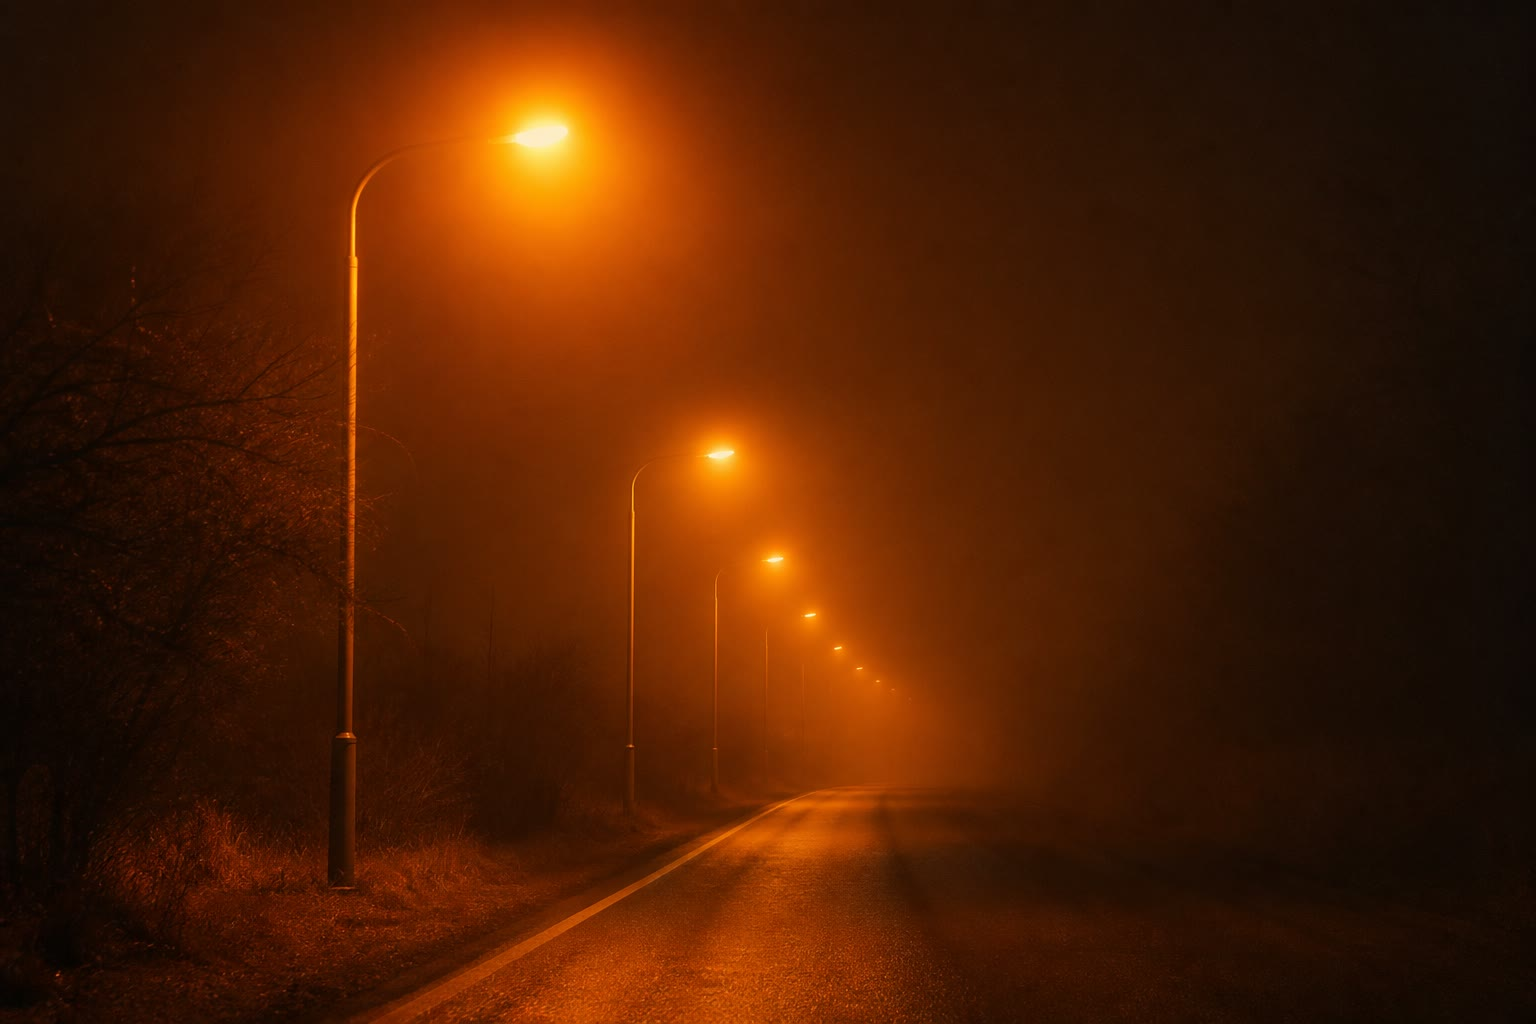
\includegraphics[width=0.58\linewidth]{images/book4/ai/b4-18-sodium-lamps-fog.jpg}

{\small 雾中的低压钠灯：单一黄色谱线，\omterm{prop:b2:scalar-light-model:coherence}{相干长度}为厘米量级——光学实验室的经典光源，也是旧街道的常客。}
\end{omfigure}

\section{问题：钠灯与激光笔}

\begin{problem}[{周末问题——拆解两种光源：
旧街道的黄色钠灯、报告厅里的红色激光笔，
以及决定各自能否产生条纹的那一个数}]
\label{pb:b2:scalar-light-model:1}

\medskip
\noindent\textbf{第一部分——钠灯。}
钠发出黄色双线，$\lambda_1 = \qty{589.0}{nm}$，$\lambda_2 =
\qty{589.6}{nm}$。每条谱线的固有宽度为 $\Delta\nu_{\text{自然}} =
\qty{10}{MHz}$；灯中原子温度为 \qty{500}{K}（钠的质量为
\qty{23}{u}，$k_B = \qty{1.38e-23}{J/K}$，$u = \qty{1.66e-27}{kg}$）。
\begin{enumerate}
  \item 两条谱线的频率及其差。
  \item 若只计入固有宽度，单条谱线的
        \omterm{prop:b2:scalar-light-model:coherence}{相干长度}。
  \item 多普勒展宽：沿视线以速度 $v$ 运动的原子
        发出 $\nu(1 + v/c)$ 的光；取沿一个轴的热运动方均根速率 $\sqrt{k_BT
        /m}$，估计 $\Delta\nu_D$，并与
        固有宽度比较。
  \item 多普勒展宽后单条谱线的\omterm{prop:b2:scalar-light-model:coherence}{相干长度}；在实际的
        高压灯中，碰撞使谱线再展宽十倍：
        求此时的\omterm{prop:b2:scalar-light-model:coherence}{相干长度}。
  \item 两条谱线合在一起：路程差多大时，它们的
        条纹系统由重合变为反相，再回到重合
        （“拍长”$\lambda^2/\Delta\lambda$）？共有多少条条纹？
  \item 一名学生用这盏灯搭建双光束干涉仪，
        使路程差从零开始增加：描述
        所见对比度的变化——拍现象与最终消光，结合
        求得的数值。
  \item 这盏灯辐射 \qty{1}{W} 黄光：每秒光子数；
        单个光子的能量（以 eV 计），以及光为何呈黄色。
  \item 两盏钠灯并排放置：它们的光能否干涉？
        对同一盏灯的两条谱线，为何问题不同？
\end{enumerate}

\medskip
\noindent\textbf{第二部分——激光笔。}
一支 \qty{1}{mW} 的红色二极管激光器，波长 \qty{650}{nm}，若价格低廉，其发出的光包含若干
分布在 $\Delta\lambda = \qty{0.5}{nm}$ 范围内的纵模；稳频的
单模激光器则有 $\Delta\nu = \qty{1}{MHz}$。
\begin{enumerate}[resume]
  \item 两支激光笔的\omterm{prop:b2:scalar-light-model:coherence}{相干长度}。
  \item 每秒发出的光子数；沿光束方向光子间的平均间距
        （以米计）；与\omterm{prop:b2:scalar-light-model:coherence}{相干长度}比较——
        这说明了关于“光子干涉”的什么？
  \item 将 \qty{0.5}{nm} 的展宽换算为频率宽度；二极管
        的谐振腔长 \qty{1}{mm}，$n = 3.5$：求其
        纵模间距（$c/2nL$），以及展宽内的
        模式数。
  \item 光束（直径 \qty{1}{mm}）射到一个光电二极管上，
        每个光子产生一个电子：求电流。
  \item 将低价激光笔用于路程差为
        \qty{2}{mm} 的双光束干涉仪：是否出现条纹？稳频的
        激光器路程差为 \qty{10}{m} 时又如何？
  \item 二极管的输出实际上以
        \qty{1}{ns} 的脉冲开启和关闭：相邻两个周期的脉冲
        能否相互干涉？这里决定相干性的，是
        脉冲长度，还是谱线宽度？
  \item 为何激光在墙上看起来呈“斑点”状，
        而灯光却没有？
  \item 波长为 \qty{650}{nm} 的红色发光二极管，$\Delta\lambda = \qty{25}{nm}$：\omterm{prop:b2:scalar-light-model:coherence}{相干
        长度}是多少？为何一些投影仪偏爱发光二极管而非激光器？
\end{enumerate}

\medskip
\noindent\textbf{第三部分——\omterm{def:b2:scalar-light-model:path}{光程}与探测器。}
\begin{enumerate}[resume]
  \item 在干涉仪的一臂中插入厚 \qty{2}{mm} 的玻璃片（$n = 1.5$）；
        求附加\omterm{def:b2:scalar-light-model:path}{光程}，以及
        越过标记的条纹数。
  \item 将玻璃片倾斜 \qty{10}{\degree}：求附加\omterm{def:b2:scalar-light-model:path}{光程}（玻璃中的长度取 $e/\cos r$
        ，减去其所取代的空气部分，一级近似为
        $e(n/\cos r - \cos(i - r)/\cos r)$——或直接
        用较长的几何路径估计）；求条纹移动量的
        数量级。
  \item 探测器为照相机，像素为 \qty{10}{\micro m}；条纹
        间距为 \qty{50}{\micro m}：每条条纹占多少像素，
        以及若间距降至
        \qty{10}{\micro m}，测得的对比度会怎样变化？
  \item 在一个像素上以 \qty{1}{\micro W/cm^2} 曝光 \qty{10}{ms}：每
        像素的光子数；相对光子噪声。
  \item 两束强度均为 $I_0$ 的相干等幅波，路程差为
        $\delta$ 处相遇：写出光强 $I(\delta)$ 以及
        条纹在 $\delta$ 中的周期。
  \item 条纹以 \qty{1}{kHz} 的速率掠过某一点（由振动的
        镜子引起）：眼睛看到什么，光电二极管看到什么？
  \item 干涉仪的两臂穿过 \qty{10}{m} 的空气（$n - 1 =
        \qty{2.9e-4}{}$）：以条纹数计的超出真空的\omterm{def:b2:scalar-light-model:path}{光程}；
        空气压强变化 \qty{1}{\%} 对图样的影响。
  \item 灯与激光笔给出相同的 \qty{1}{\micro W/cm^2}：哪一个
        每秒给出更多光子？为何这对
        条纹无关紧要？
  \item 总结：对每种光源，给出其\omterm{prop:b2:scalar-light-model:coherence}{相干长度}、限制它的因素，
        以及它允许的干涉仪路程差。
\end{enumerate}
\end{problem}
